
% ***************************************************
% Example of an internal chapter
% ***************************************************
%This is an internal chapter of the thesis.
%If you have a long title, you can supply an abbreviated version to print in the Table of Contents using the optional argument to the \chapter command.
\chapter[Results]{Results}
\label{chap:Results}	%CREATE YOUR OWN LABEL.
\pagestyle{headings}


The presented design provides a number of extensible blocks which can be configured to implement a simple convolutional neural network, or use the convolutional core to accelerate other image-processing algorithms. 
This chapter analyses the practicality of the design by assessing the throughput, resource utilisation and timing of the design.
The design is compared against CPU and GPU implementations to demonstrate the speedup to utilisation ratio, when compared to software-based implementations.

\section{Latency and Throughput}

Image processing algorithms are a prime candidate for hardware acceleration due to the large amount of data and the need for parallel processing.
This fundamentally makes reducing the latency of the design imperative, as outlined in section \ref{sec:convolution} - making this a critical metric for the design.
Latency is directly proportional to the number of clock cycles required to process the input image, and hence dictates the throughput of the design.

By developing the design at a hardware level, this allows for time deterministic performance, where the latency is known based on the convolution parameters.
The three designs presented in section \ref{sec:convolution} will require differing number of clock cycles, due to the varying levels of parallellisation to accomodate the varying FPGA resources.

\subsection{Time Determinism}
The advantage of an FPGA is the ability to implement the design at a hardware level, allowing for time deterministic performance.
As there are no overheads from the CPU or GPU, the latency is known based on the convolution parameters.
This allows for the latency to be determined at synthesis time, and the throughput to be calculated based on the number of clock cycles required to process the input image.

The fully parallel convolution implementation is constant, and will always require a single clock cycle to complete the operation \ref{eq:fully_parallel}.
\begin{equation}
    T_{fully\ parallel} = 1 \label{eq:fully_parallel}
\end{equation}

The partially folded implementation is dependent on the size of the kernel, and the stride. 
The image size is mutated by the size of the zero padding.
The defined variables can be found in table \ref{tab:convolution_parameters}.

\begin{equation}
    T_{partially\ folded} = \left( \frac{I + 2Z - K}{s} + 1 \right)^2 \times O
\end{equation}

The fully folded implementation is dependent on the same parameters, however, the kernel size is the primary driver for the number of clock cycles required.

\begin{equation}
    T_{fully\ folded} = K^2 \times C \times \left( \frac{I - K}{S} + 1 \right)^2 \times O
\end{equation}

\subsection{Implementation Timing}
The time deterministic nature of the FPGA allows for the timing of the design to be known at synthesis time.
This is in contrast to the CPU and GPU, where the timing is dependent on the computational workload and the underlying hardware.
Executing the design on an FPGA for the selected machine learning core parameters, the timing characteristics are as follows:

\begin{table}[h!]
    \centering
    \caption{Latency and throughput comparison of convolutional core implementations}
    \label{tab:latency_comparison}
    \begin{tabular}{lcccc}
        \toprule
        Implementation & Clock Cycles & Latency (ns) & Throughput (images/s) \\
        \midrule
        No Folding & 1 & 10 & 10e8 \\
        Partially Folded & 490 & 4900 & 2.04e5 \\
        Fully Folded & 1960 & 19600 & 5.1e4 \\
        \bottomrule
    \end{tabular}
\end{table}

There is a non-linear relationship between the level of folding and the latency of the design.
This is due to the increased number of MAC units required to process the input image, and the increased control logic required to manage the dataflow depending on the degree of folding.
The latency is computed based on the implementable design, where route and place succeeds - a clock speed of 100MHz is used for the FPGA.


\subsection{Comparison}
The performance characteristics of hardware-based convolution implementations can be evaluated against traditional computing platforms to understand their relative strengths and trade-offs. As discussed in section \ref{sec:platforms}, GPUs leverage thousands of CUDA cores for parallel processing, while CPUs rely on fewer but more complex processing units.

The NVIDIA Tesla P100 and A100 GPUs were selected as representative high-performance computing platforms, featuring dedicated hardware for parallel matrix operations. The P100 utilizes 3584 CUDA cores with 16GB of HBM2 memory, while the A100 represents NVIDIA's more recent architecture with 6912 CUDA cores and 40GB of memory (specifications detailed in \ref{app:device_information}). 
Relatively, the more modern A100 GPU provides is expected to provide an 11x speedup over the P100 - as shown in figure \ref{fig:nvidia}.
A standard Intel i7 CPU provides the baseline for comparison.

\begin{figure}[h]
    \centering
    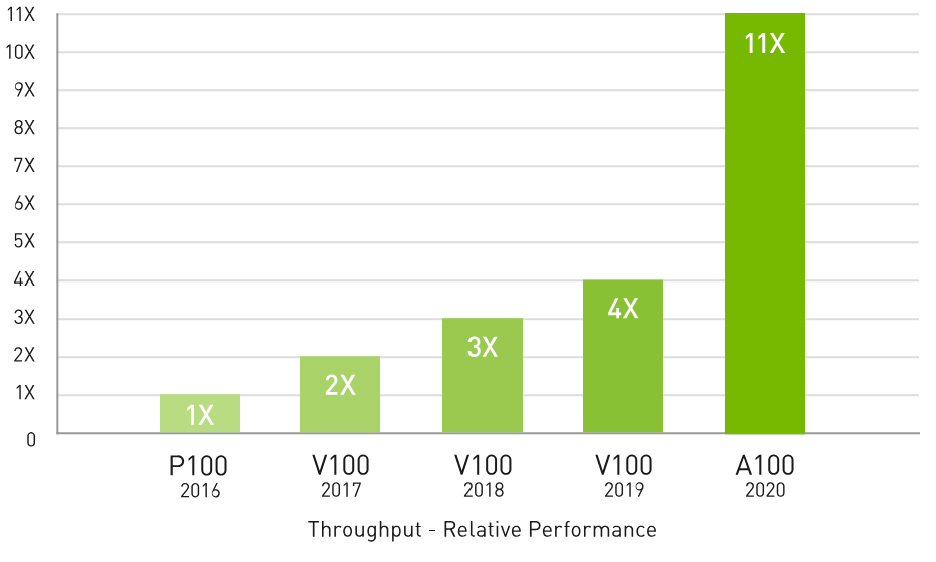
\includegraphics[width=0.75\textwidth]{nvidia.png}
    \caption{Comparison of relative performance of Nvidia GPUs \cite{23}.}
    \label{fig:nvidia}
\end{figure}

The performance comparison between implementations is presented in Table \ref{tab:platform_comparison}, which reveals several key insights:

\begin{itemize}
    \item The no-folding FPGA implementation achieves remarkable single-cycle latency (10ns), demonstrating the potential of fully parallel hardware implementations
    \item GPU implementations show strong performance, with the A100 achieving 609ns latency compared to the P100's 1020ns
    \item CPU implementation exhibits significantly higher latency at 229,782ns, highlighting the limitations of sequential processing
    \item The partially and fully folded FPGA implementations fall between CPU and GPU performance, with latencies of 4900ns and 19600ns respectively
\end{itemize}

This can be equally represented in terms of throughput, as shown in Table \ref{tab:latency_comparison}, as reducing the latency of convolution directly translates to an increase in throughput.
The throughput provides a more human-readable representation of the performance.

To provide context for these hardware implementations, Table \ref{tab:platform_comparison} compares their performance against traditional computing platforms:

\begin{table}[h!]
    \centering
    \caption{Platform comparison of latency and throughput}
    \label{tab:platform_comparison}
    \begin{tabular}{lcc}
        \toprule
        Device & Latency (ns) & Throughput (images/s) \\
        \midrule
        CPU (Intel i7) & 229782 & 4.35e3 \\
        Fully Folded & 19600 & 5.1e4 \\
        Partially Folded & 4900 & 2.04e5 \\
        Nvidia Tesla P100 GPU & 1020 & 9.8e6 \\
        Nvidia A100 GPU & 609 & 1.64e6 \\
        No Folding & 10 & 10e8 \\
        \bottomrule
    \end{tabular}
\end{table}

When considering throughput, the results demonstrate even more dramatic differences. 
The no-folding implementation theoretically achieves 10e8 images/s, though this is not practically achievable due to resource constraints. The GPU implementations demonstrate impressive real-world throughput, with the P100 processing 9.8e6 images/s and the A100 achieving 1.64e6 images/s. The CPU implementation manages only 4.35e3 images/s, while the partially folded and fully folded FPGA implementations achieve 2.04e5 and 5.1e4 images/s respectively.
The logarithmic scale of the throughput is provided in figure \ref{fig:throughput_comparison}.

\begin{figure}[h]
    \centering
    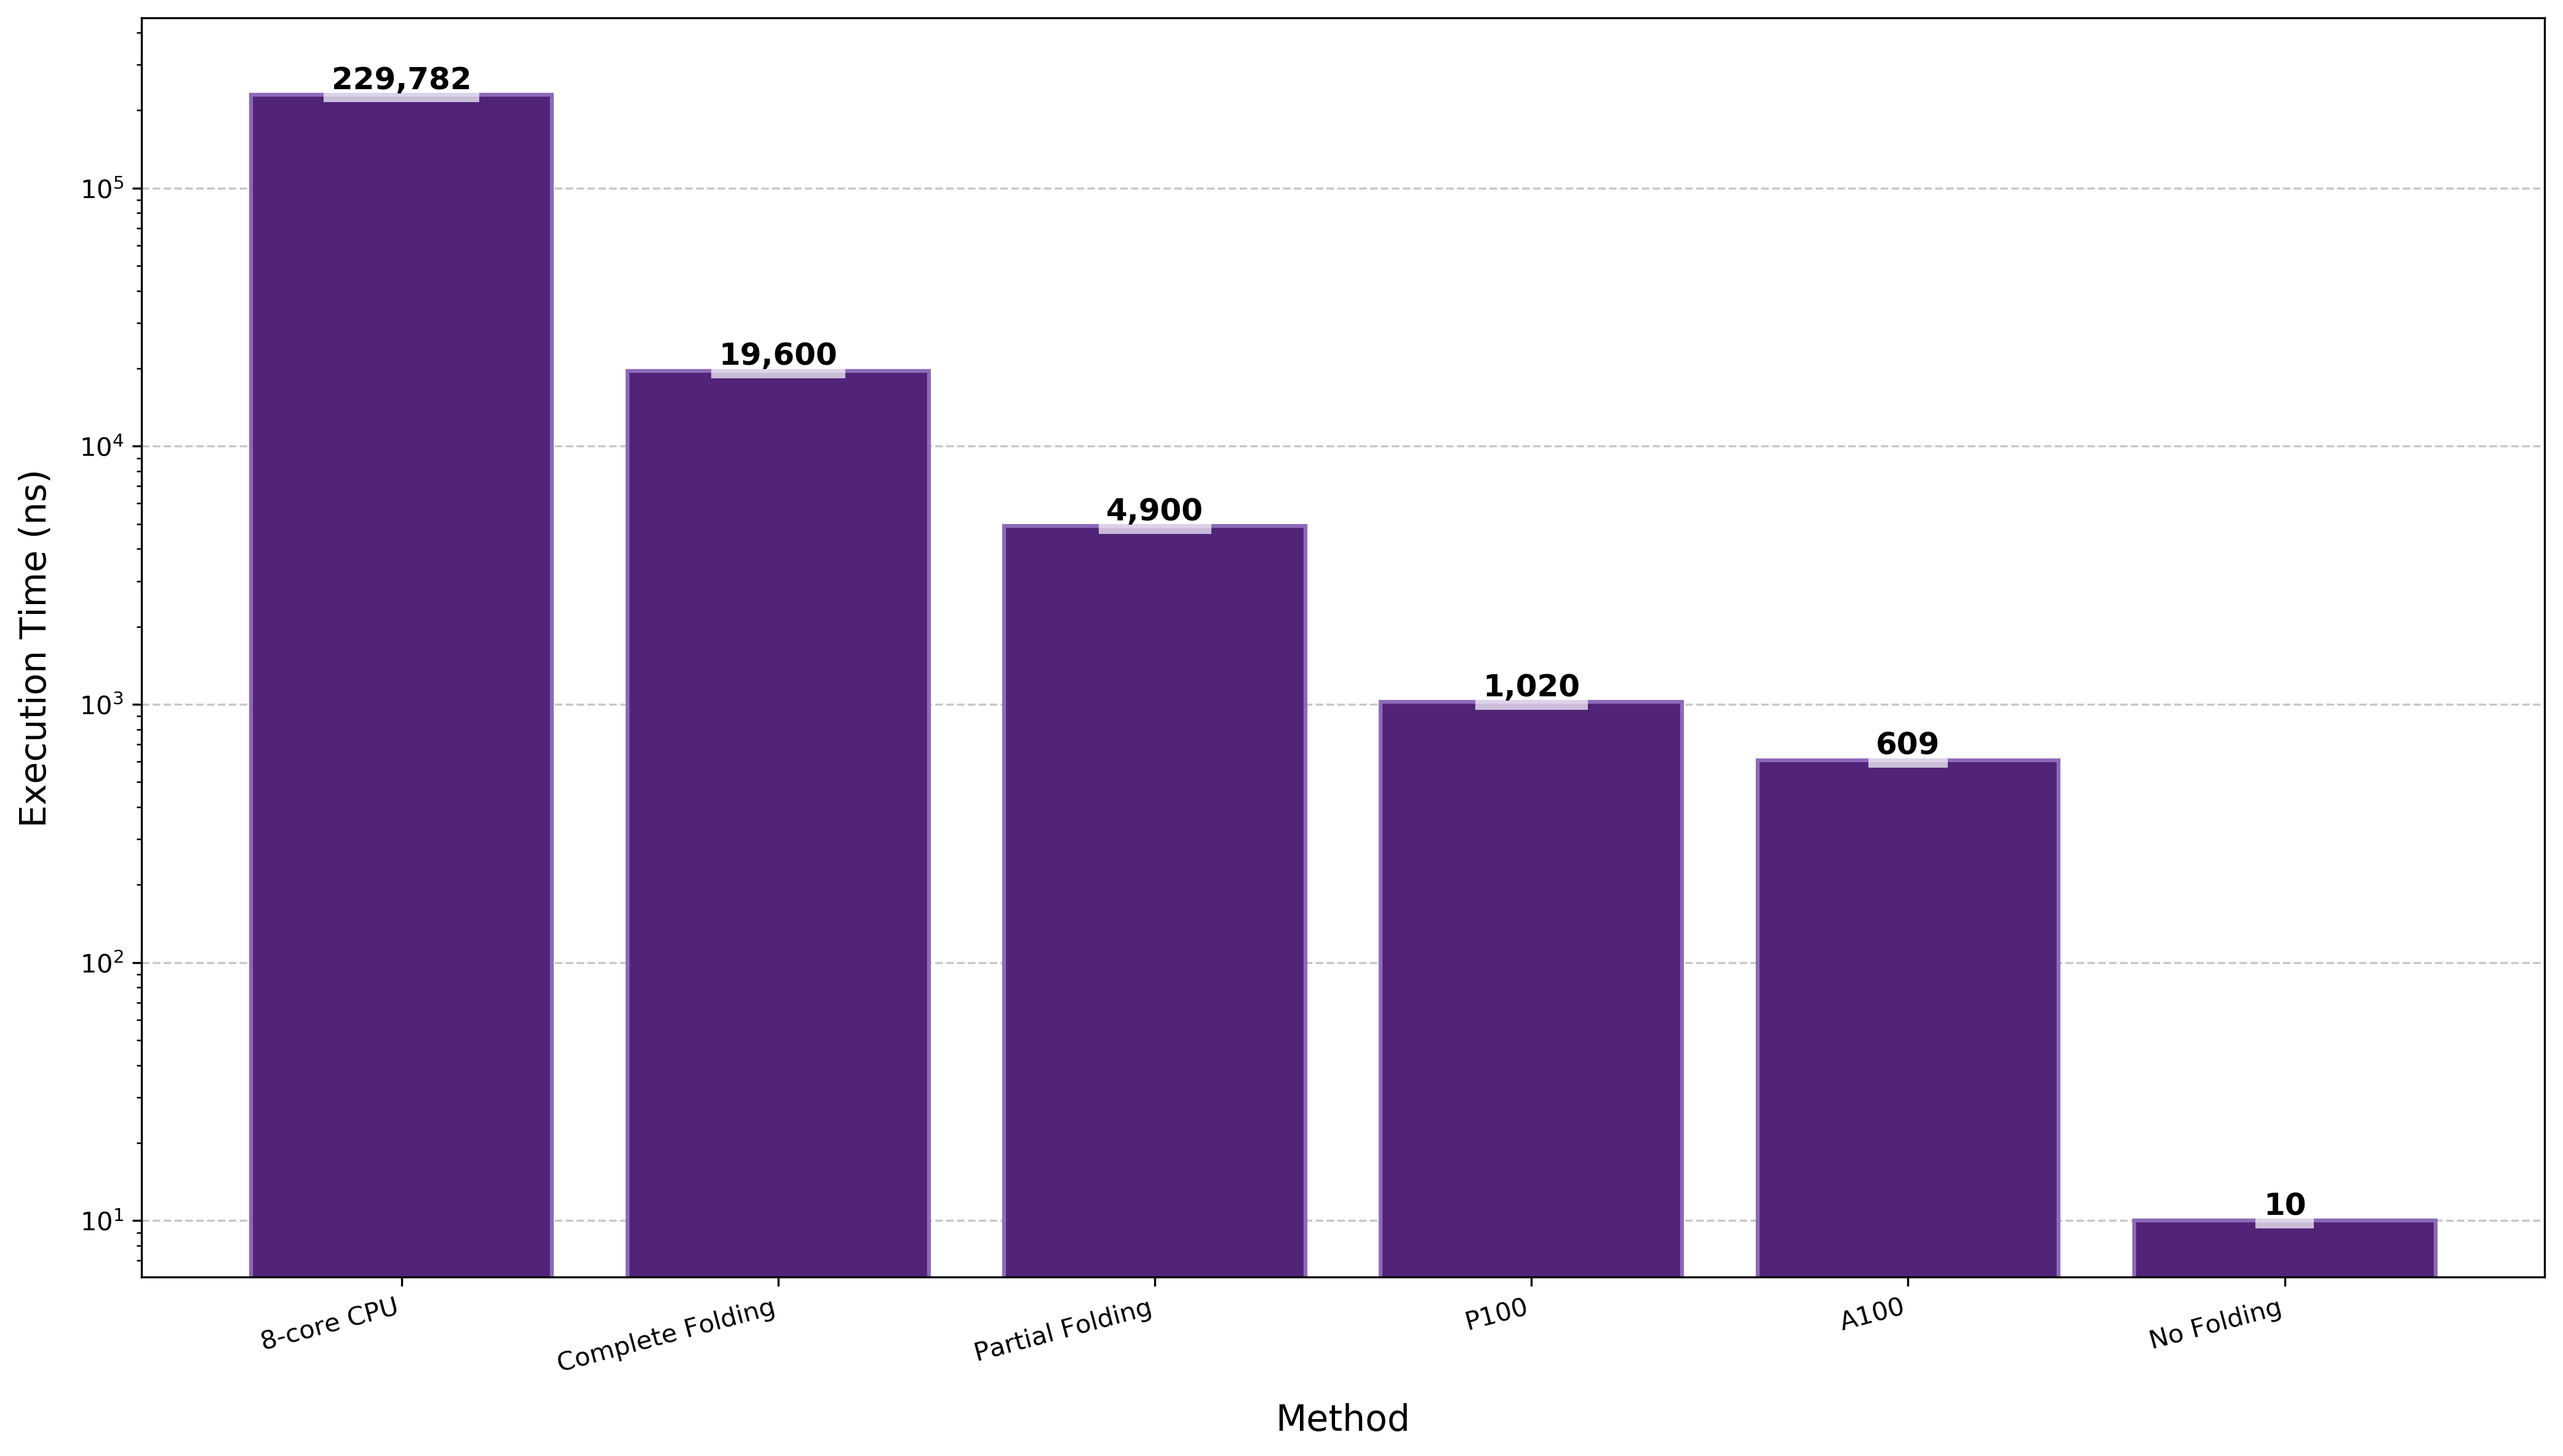
\includegraphics[width=0.75\textwidth]{chart_ex_time.png}
    \caption{Logarithmic scale of the latency of the design against the CPU and GPUs selected.}
    \label{fig:throughput_comparison}
\end{figure}
These results demonstrate that while FPGAs cannot match the absolute performance of modern GPUs for convolution operations, they offer significant advantages over CPU implementations while maintaining lower power consumption and cost compared to GPU solutions. This positions FPGA implementations as particularly suitable for embedded and edge computing applications where power efficiency and cost are primary concerns.

\clearpage
\section{Accuracy}
Hardware implementations of convolution operations must balance resource utilisation against computational precision. Enable time multiplexing (referred to as folding) is used to separate the input image over different time intervals to reduce the number of MAC units required for processing. While this approach effectively reduces hardware resource consumption, it introduces potential sources of computational error not present in software implementations.

At a hardware layer, the accuracy between software and hardware implementations can vary due to several factors:
\begin{itemize}
    \item The precision of the data types used in the design
    \item The potential for overflow or underflow in arithmetic operations
    \item The accumulation of rounding errors in sequential computations
\end{itemize}

\begin{figure}[h]
    \centering
    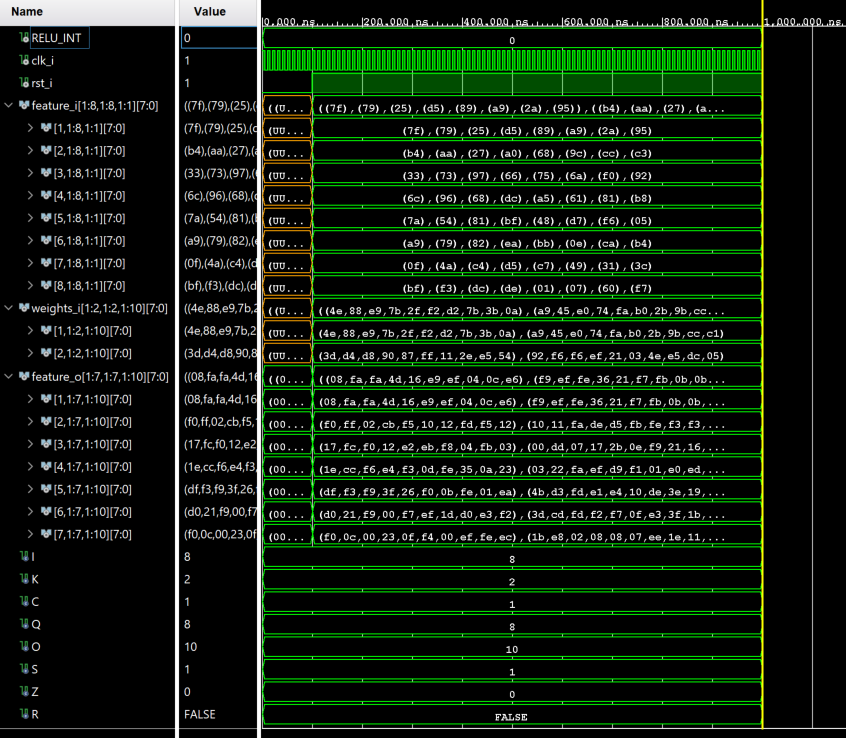
\includegraphics[width=0.9\textwidth]{tb_conv.png}
    \caption{Simulation waveform demonstrating fully parallelised implementation timing.}
    \label{fig:sim_parallel}
\end{figure}

To validate the accuracy of the design, a pseudo-random generator is used to prevent bias in the image and the weights. A testbench is then employed to simulate the operation of the design, and compare the output against the expected result using a software-based implementation for verification.

Figure \ref{fig:sim_parallel} provides a simulation waveform demonstrating the timing of the fully parallel implementation. When the setup time is complete, the output is available on the next clock cycle. This implementation requires minimal control logic, with its behavior primarily determined by the number of MAC units and the kernel size. As expected, the fully parallel implementation achieves the highest accuracy, completing operations in a single clock cycle with no detectable error when compared against the software reference.

The partially folded and folded implementations share the same approach for handling the dataflow component. However, analysis reveals a single error in one MAC operation present in both folding designs. While this introduces a small deviation from the expected results, the timing characteristics remain unaffected, with operations completing in the expected number of clock cycles. Figure \ref{fig:sim_partial} shows the simulation waveform for the partially folded implementation, demonstrating the trade-off between resource utilisation and computational precision.

\begin{figure}[h]
    \centering
    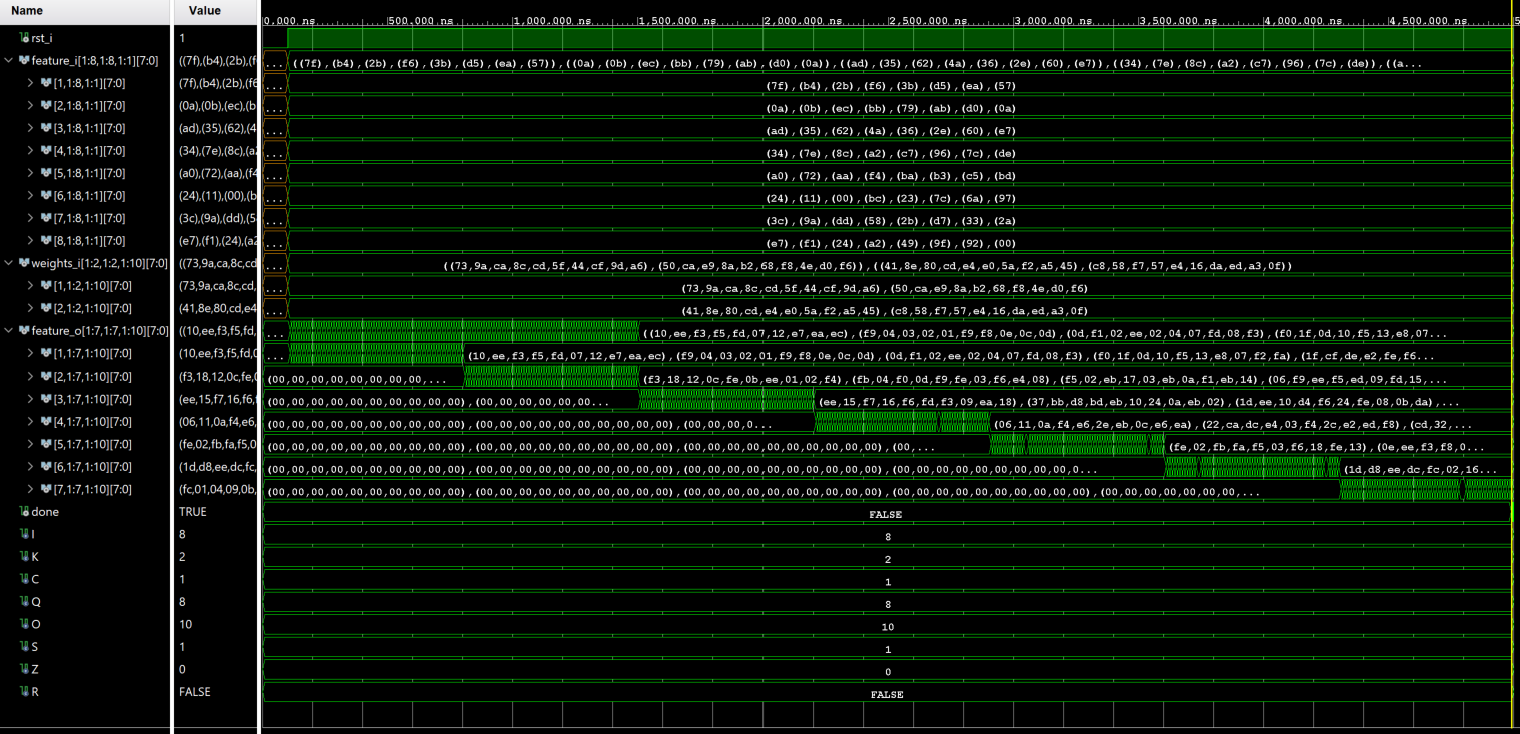
\includegraphics[width=0.9\textwidth]{tb_conv_folded.png}
    \caption{Simulation waveform demonstrating partially folded implementation timing.}
    \label{fig:sim_partial}
\end{figure}

\section{Resource Utilisation}
Resource utilisation is an integral part in validating the feasibility of implementing the design on a particular FPGA or microchip, due to the limited resources available. The three implementation approaches demonstrate distinct trade-offs between parallelization and hardware requirements, each suited to different application constraints.

\subsection{Hardware Requirements}
The number of hardware multipliers and adders required for each implementation are deterministic, similar to that of the clock cycles required.
This directly translates to the number of LUTs required for the design.

For the sequential MAC of the fully parallelised implementation, the number of multipliers is dependent on the kernel size as this determines the number of operations required.

\begin{equation}
    M_{fully\ parallel} = K^2 \times C \times O
\end{equation}

The adders will be one less than the number of multipliers, as the final operation does not require an adder.

\begin{equation}
    A_{fully\ parallel} = M_{fully\ parallel} - 1
\end{equation}

For the partially folded implementation, the adders and multipliers are shared across time. 
This allows for an independency from the number of output channels, as the number of operations is fixed by the kernel size.

\begin{equation}
    M_{partially\ folded} = K^2
\end{equation}

\begin{equation}
    A_{partially\ folded} = K^2 - 1
\end{equation}

A fully folded implementation will only require a single MAC unit, as all operations are performed sequentially. Hence, a constant number of both adders and multipliers are required with a value of 1 - independent of the kernel size.
\begin{equation}
    M_{fully\ folded} = 1
\end{equation}

\begin{equation}
    A_{fully\ folded} = 1
\end{equation}

\subsection{Implementation}
The resource utilisation across implementations demonstrates the trade-offs between parallelization and FPGA resource consumption. Table \ref{tab:resource_comparison} shows the percentage utilisation of key FPGA resources for each design variant.

\begin{table}[h!]
    \centering
    \caption{Resource utilisation comparison of convolutional core implementations}
    \label{tab:resource_comparison}
    \begin{tabular}{lcccc}
        \toprule
        Implementation & LUTs & Registers & F7 Muxes & F8 Muxes \\
        \midrule
        No Folding & 144061 (692.60\%) & 3430 (8.25\%) & 0 (0\%) & 0 (0\%) \\
        Partially Folded & 1622 (7.8\%) & 3456 (8.31\%) & 0 (0\%) & 0 (0\%) \\
        Fully Folded & 2551 (12.26\%) & 9511 (23.10\%) & 592 (3.63\%) & 240 (2.94\%) \\
        \bottomrule
    \end{tabular}
\end{table}

The no-folding implementation represents a fully parallelized approach, where all operations are performed simultaneously. While this achieves optimal performance, the resource requirements (692.60\% of available LUTs) make it impractical for implementation on most FPGAs. This demonstrates the fundamental limitation of full parallelization: the hardware requirements scale linearly with the size of the convolution operation.

The partially folded implementation introduces time multiplexing through dataflow control logic, significantly reducing hardware requirements to just 7.8\% of available LUTs. This dramatic reduction comes with minimal overhead in control logic, representing an efficient compromise between resource utilisation and performance.

Interestingly, the fully folded implementation, despite using only a single MAC unit, shows higher resource utilisation (12.26\% LUTs) than the partially folded approach. This counter-intuitive result stems from the complex control logic required to manage the sequential processing of operations. The additional registers (23.10\%) and multiplexers (F7: 3.63\%, F8: 2.94\%) needed for control flow management effectively negate the resource savings from reduced MAC units.

These results demonstrate that aggressive resource optimization through full folding may not always yield the most efficient implementation. The partially folded architecture achieves a better balance, significantly reducing resource requirements while maintaining manageable control complexity.

\section{Efficiency}
As noted, the produced hardware designs are markedly slower than the GPU implementations.
However, this is not an even comparison, due to the differing hardware resources available.
Hence, it is more effective to provide the metric for the convolutional cores using an efficiency metric instead of pure throughput.
To quantify implementation efficiency, we define a metric that relates performance to resource utilisation.

\begin{equation}
    \text{Efficiency} = \frac{\text{Throughput (images/s)}}{\text{LUT Utilization (\%)}}
\end{equation}

\begin{table}[h!]
    \centering
    \caption{Efficiency comparison of convolutional core implementations}
    \label{tab:efficiency_comparison}
    \begin{tabular}{lcccc}
        \toprule
        Implementation & Efficiency \\
        \midrule
        No Folding & 10e8 \\
        Partially Folded & 26153.8 \\
        Fully Folded & 4159.9 \\
        \bottomrule
    \end{tabular}
\end{table}


This metric reveals that the partially folded implementation achieves an efficiency of 26,153.8, significantly outperforming the fully folded design's efficiency of 4,159.9. This substantial difference in efficiency (6.29x) demonstrates that the partially folded architecture strikes an optimal balance between resource utilisation and performance for the target application.

While GPU implementations achieve superior absolute throughput, with the Tesla P100 processing 9.8e6 images/second, they represent a fundamentally different point in the design space, optimized for high-performance computing rather than embedded applications. The partially folded FPGA implementation offers a more appropriate solution for resource-constrained environments, providing a 46.9x speedup over CPU implementation while maintaining modest resource requirements.

These results demonstrate that the relationship between folding factor and implementation efficiency is non-linear, with the partially folded architecture representing a local optimum in the design space. This finding has significant implications for future FPGA-based CNN accelerator designs, suggesting that moderate levels of resource sharing can achieve better overall system efficiency than either extreme of the folding spectrum.

\section{RISC-V processor}
The NeoRV32 processor consumed little of the hardware resources, as it effectively acts as a method to memory map a peripheral such that the convolution or machine learning cores can access the location of an input image.
Communication is implemented with a 32-bit wide wishbone interface, and a buffer used to ingest the data to the core.
The usage of the RISC-V processor is provided in table \ref{tab:riscv_usage}.

\begin{table}[h!]
    \centering
    \caption{Usage of the RISC-V processor}
    \label{tab:riscv_usage}
    \begin{tabular}{lccc}
        \toprule
        Resource & Used & Available & Utilization (\%) \\
        \midrule
        LUTs & 1934 & 20800 & 9.30\% \\
        Registers & 1350 & 41600 & 3.25\% \\
        F7 Muxes & 1 & 16300 & 0.006\% \\
        F8 Muxes & 0 & 8150 & 0\% \\
        \bottomrule
    \end{tabular}
\end{table}

Equally, the processor can interface via a memory mapped interface to the convolutional cores.
Common designs employ camera modules directly on the FPGA, which require BRAM to store the incoming image data.
This can be used to abstract away from the use of a 32-bit wide wishbone interface, and instead use a memory mapped interface to the convolutional cores.
The NeoRV32 processor can then be used as a controller to start the convolution operation, and to retrieve the output signal. 

\section{Quantisation}
The quantisation of the weights allows for truncating of the number of bits used to represent the weights, which in turn reduces the resources required for implementing the convolution operation. As demonstrated in the design phase, for the given neural network, this is a mostly lossless operation, with a negligible impact on the accuracy of the network.

The effectiveness can be computed based on the utilisation of the FPGA resources when compared to the baseline design. The model was reconstructed using 2, 4, 8 and 16 bit precision weights to compare the utilisation of the FPGA resources on the unfolded convolution core.

\begin{table}[h]
    \centering
    \caption{Utilisation of the FPGA resources when compared to the baseline design.}
    \label{tab:quantisation_utilisation}
    \begin{tabular}{lcccc}
        \toprule
        Bit Quantisation & LUTs & Registers \\
        \midrule
        2-bit & 11033 (53.04\%) & 980 (2.36\%) \\
        4-bit & 44591 (214.38\%) & 1960 (4.71\%) \\
        8-bit & 144061 (692.60\%) & 3430 (8.25\%) \\
        16-bit & 570540 (2742.98\%) & 7510 (18.05\%) \\
        \bottomrule
    \end{tabular}
\end{table}

The results demonstrate significant resource savings through weight quantisation. Reducing precision from 16-bit to 8-bit yields a 4x reduction in LUT utilisation (from 2742.98\% to 692.60\%). Further reduction to 4-bit provides an additional 3.2x improvement, while 2-bit quantisation achieves a 13x reduction compared to the 8-bit baseline.

This dramatic reduction in resource utilisation is achieved by performing quantisation during the training phase, where the network learns to operate with reduced precision weights. The hardware implementation then benefits from these smaller bit widths without requiring additional computation for runtime quantisation.

In hardware, these quantised operations can be efficiently implemented through bit shifting operations. For example, multiplication by powers of 2 can be achieved through left shifts, while division can be implemented through right shifts. This approach eliminates the need for complex floating-point arithmetic units, further reducing hardware complexity and improving performance. The general form for this operation can be expressed as:

\begin{equation}
    result = input \ll n
\end{equation}

Where $n$ represents the number of bit positions to shift, and $\ll$ denotes a left shift operation.

The trade-off between precision and resource utilisation becomes particularly apparent when examining the register usage. While LUT consumption scales exponentially with bit width, register utilisation shows a more linear relationship, suggesting that control logic overhead remains relatively constant across different quantisation levels.

These findings indicate that aggressive quantisation (2-bit or 4-bit) can make otherwise impractical designs feasible on resource-constrained FPGAs, provided the application can tolerate the associated reduction in numerical precision. For many neural network inference tasks, this trade-off is acceptable, as modern training techniques can compensate for reduced precision through appropriate weight adjustment during the training phase.
This is the basis of binarized neural networks, which provide a single-bit precision to substantially compress the neural network at the training level \cite{18}.

\section{Extensibility}
The project aims to provide a flexible design that can be extended to support other machine learning algorithms. While the core components of neural networks - convolution, pooling, and fully connected layers - all fundamentally rely on MAC operations, their direct implementation often exceeds available FPGA resources. This section explores the practical considerations and solutions for implementing these components on resource-constrained hardware.

\subsection{Resource Constraints}
Without folding techniques, the implementation of a complete neural network becomes impractical on most FPGAs. This is particularly evident in fully connected layers, which require a MAC unit for each input-weight combination. For example, a fully connected layer with 1024 inputs and 10 outputs would require 10,240 MAC units - far exceeding the resources of typical FPGAs.

The solution lies in applying appropriate folding strategies to each layer type:
\begin{itemize}
    \item Convolution layers can utilize partial folding to balance parallelism and resource usage
    \item Pooling operations can share MAC units through time multiplexing
    \item Fully connected layers require aggressive folding due to their dense computation requirements
\end{itemize}

\subsection{Implementation Architecture}
The described machine learning core was synthesised and implemented on the Digilent Basys 3 board, employing a RISC-V softcore processor to interface with the FPGA fabric. This allows for the design to be easily extended to support other machine learning algorithms, by utilising the same interface.

The testbench for this is illustrated in figure \ref{fig:tb_extensibility}. There is a significant initial setup time required to load the weights and biases into the memory, and to configure the machine learning core. However, this is a one-time operation, and only requires the RISC-V processor to be programmed. Once this is complete, the machine learning core can be used to process data streams in a time-multiplexed manner, with no additional overheads. This simulates effectively a cold-start of the machine learning core, which software implementations will also initially face.

\begin{figure}[h]
    \centering
    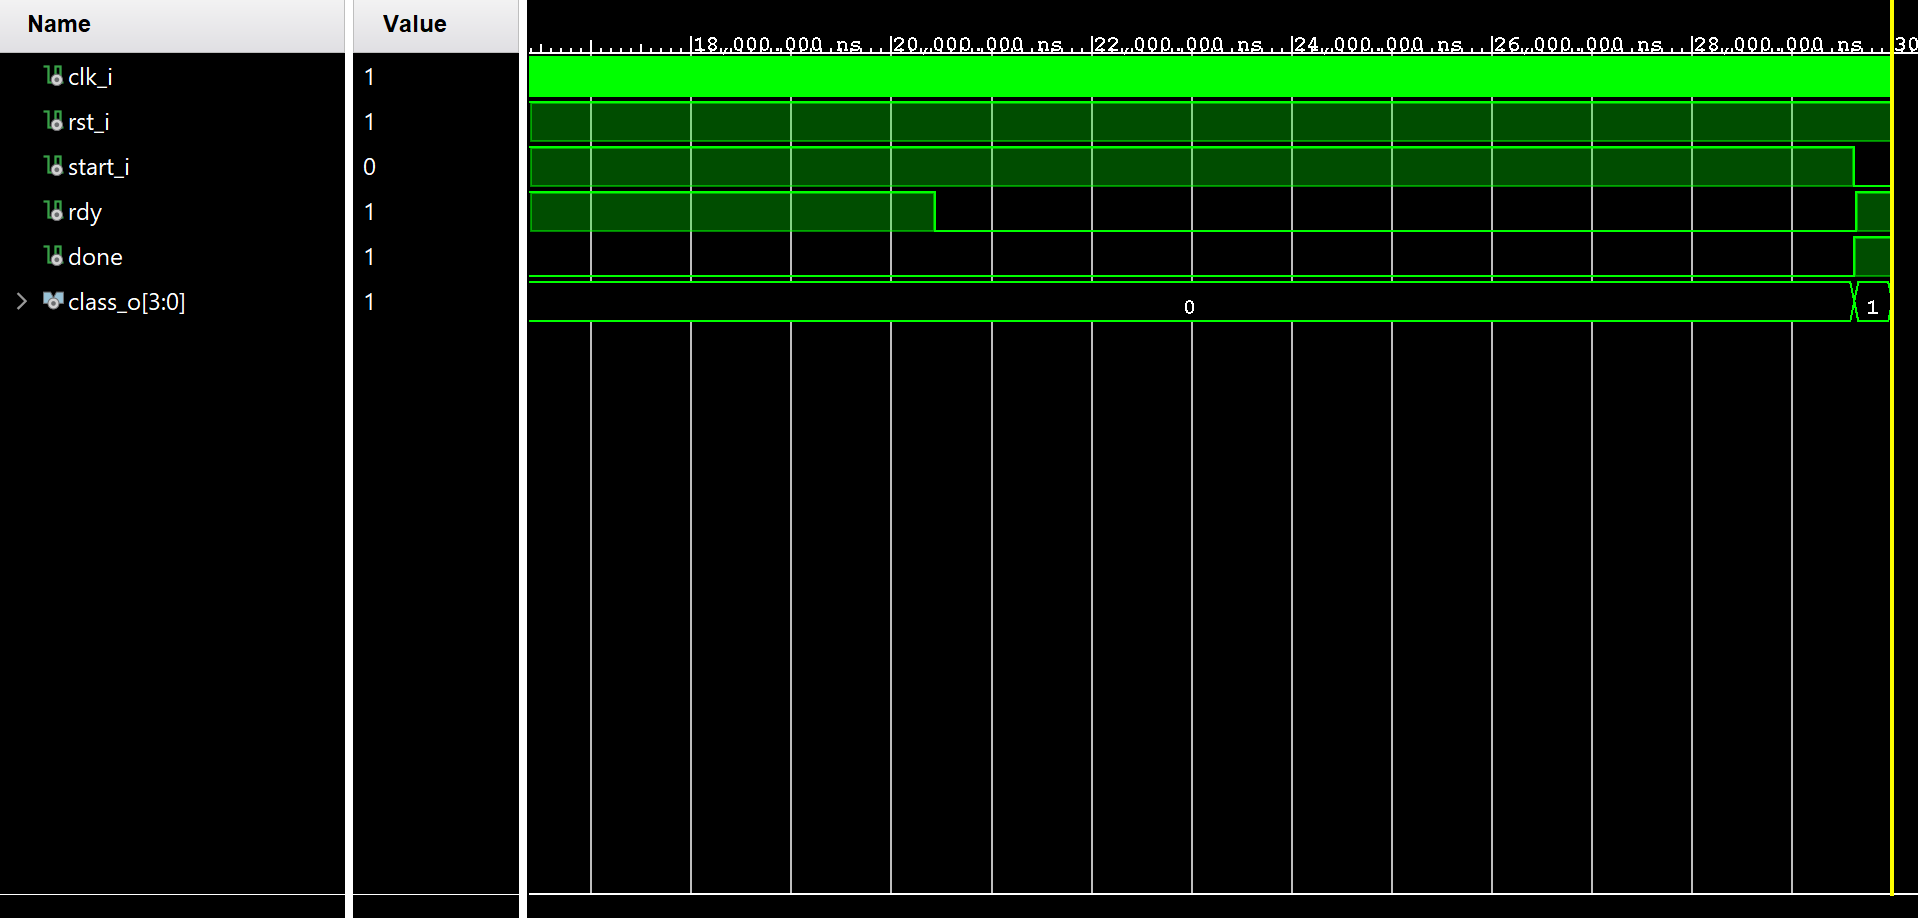
\includegraphics[width=0.9\textwidth]{tb_mem_accel.png}
    \caption{Simulation waveform demonstrating the extensibility of the design.}
    \label{fig:tb_extensibility}
\end{figure}

\subsection{Resource Sharing}
The key to implementing complex neural networks on FPGAs lies in the strategic sharing of MAC units across different layer types. By recognizing that convolution, pooling, and fully connected layers all fundamentally perform multiply-accumulate operations, a unified hardware architecture can be designed that time-multiplexes these resources effectively.

This approach offers several advantages:
\begin{itemize}
    \item Reduced resource utilization through hardware reuse
    \item Simplified control logic through standardized interfaces
    \item Flexibility to implement different network architectures
    \item Scalability to accommodate larger networks within resource constraints
\end{itemize}

The trade-off between performance and resource utilization can be dynamically adjusted through the folding factor, allowing the same design to be adapted for FPGAs with different resource constraints. This flexibility makes the architecture suitable for a wide range of applications, from edge computing devices to more capable FPGA platforms.
